\documentclass[../main.tex]{subfiles}
\begin{document}

\chapter{Metodi}

Nel lavoro svolto in questa tesi sono state prese in esame le immagini di topografia \acrshort{afm} e le ampiezze della $2^a$ e $3^a$ armonica \acrshort{ssnom}, in quanto quelle di maggior interesse, per valutare l'efficacia di diverse tecniche di riduzione del rumore su questo tipo di immagini. È importante studiare il rumore perché dipende anche dal tempo di integrazione per pixel del microscopio: impostare un periodo di tempo più alto permette di avere immagini con meno rumore a discapito di un tempo di scansione più lungo. Usare delle tecniche di riduzione del rumore su immagini ottenute con un tempo di integrazione basso, $3$ms nel caso delle immagini del dataset SSNOMBACTER, permette di aumentare la qualità delle immagini senza dover aumentare il tempo richiesto per l'acquisizione delle immagini.\cite{baiz_2025} 

\begin{figure}[ht]
	\centering
	\begin{subfigure}{0.32\linewidth}
		\centering
		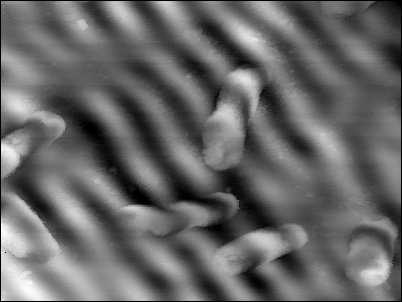
\includegraphics[keepaspectratio, width=\linewidth]{images/kp_o0a.png}
		\caption{O0A}
	\end{subfigure}
	\begin{subfigure}{0.32\linewidth}
		\centering
		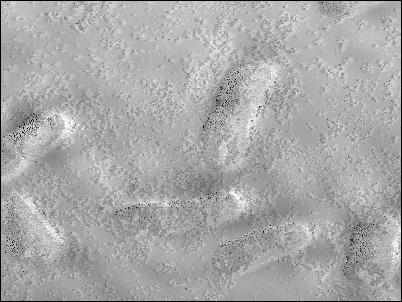
\includegraphics[keepaspectratio, width=\linewidth]{images/kp_o1a.png}
		\caption{O1A}
	\end{subfigure}
	\begin{subfigure}{0.32\linewidth}
		\centering
		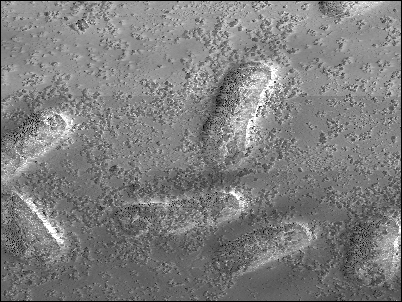
\includegraphics[keepaspectratio, width=\linewidth]{images/kp_o2a.png}
		\caption{O2A}
	\end{subfigure}\\[4pt]
	\begin{subfigure}{0.32\linewidth}
		\centering
		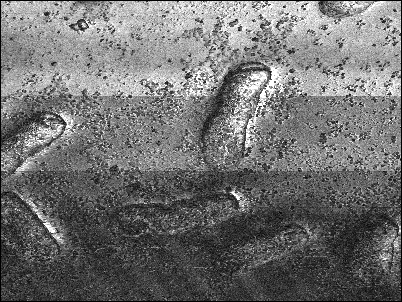
\includegraphics[keepaspectratio, width=\linewidth]{images/kp_o3a.png}
		\caption{O3A}
	\end{subfigure}
	\begin{subfigure}{0.32\linewidth}
		\centering
		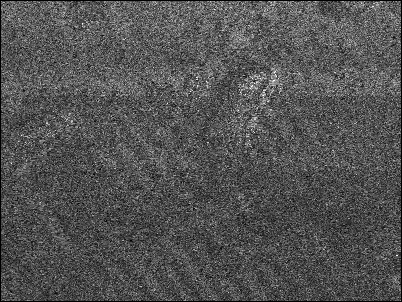
\includegraphics[keepaspectratio, width=\linewidth]{images/kp_o4a.png}
		\caption{O4A}
	\end{subfigure}
	\begin{subfigure}{0.32\linewidth}
		\centering
		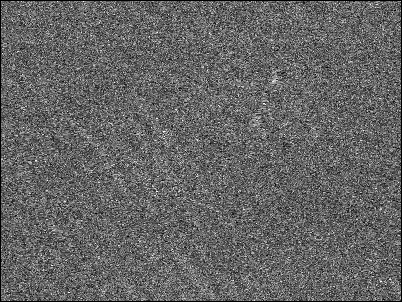
\includegraphics[keepaspectratio, width=\linewidth]{images/kp_o5a.png}
		\caption{O5A}
	\end{subfigure}
	\caption[Immagini in ampiezza SNOM di esemplari di \textit{Klebsiella pneumoniae}]{
		Immagini in ampiezza \acrshort{snom} di esemplari di \textit{Klebsiella pneumoniae} \cite{ssnombacter_data}}
\end{figure}

Nelle immagini \acrshort{ssnom}, oltre a una maggiore rilevanza dei dettagli di superficie, sono presenti diversi tipi di rumore in diverse quantità nelle immagini delle varie armoniche registrate, che invece sono assenti o molto ridotti nelle immagini di topografia.

\section{Tecniche di riduzione del rumore}

\subsection{Filtro guassiano}

Il \textbf{filtro gaussiano} è uno dei filtri più usati nell'elaborazione delle immagini ed ha applicazioni in vari campi, come tecnica di sfocatura, di riduzione del rumore e di riduzione dei dettagli. Sia nel dominio spaziale che nel dominio della frequenza, il filtro gaussiano è un filtro lineare passa-basso efficace in particolare per rimuovere il rumore soggetto a una distribuzione normale.

\begin{equation}
	G(x) = e^{-\frac{x^2}{2\sigma^2}}
\end{equation}

Il parametro $\sigma$ determina la larghezza della funzione. Nel campo dell'elaborazione delle immagini si usa una funzione gaussiana discreta con media nulla come filtro di smussamento.\cite{ito_2000}

\begin{equation}
	G[i,j] = e^{-\frac{i^2+j^2}{2\sigma^2}}
\end{equation}

Inoltre, la funzione gaussiana possiede alcune importanti proprietà: \cite{wang_2014,getreuer_2013}

\begin{enumerate}
	\itemsep0em
	\item La funzione gaussiana bidimensioname ha simmetria rotazionale. In generale, non si conosce la direzione dei bordi nelle immagini e non si può prestabilire se applicare più smussamento in una direzione rispetto all'altra prima di filtrare. Avere una simmetria rotazionale significa che il filtro gaussiano non si rivolge in nessuna direzione nelle successive elaborazioni delle immagini.
	\item La funzione gaussiana è una funzione a valore singolo. Il filtro gaussiano utilizza una media ponderata dell'intorno dei pixel per sostituire il valore del pixel centrale. Il peso è monotono decrescente con la distanza dal punto centrale quindi avrà scarso effetto sui pixel che sono lontani dal centro.
	\item La larghezza del filtro gaussiano è caratterizzata dal parametro $\sigma$. Più grande è, maggiore sarà lo smussamento e la banda di frequenza del filtro gaussiano. Regolando questo parametro di smussamento, si può ottenere un compromesso tra uno smussamento eccessiva e uno insufficiente.\\[-10pt]
	
	\begin{figure}[ht]
		\centering
		\begin{subfigure}{0.4\linewidth}
			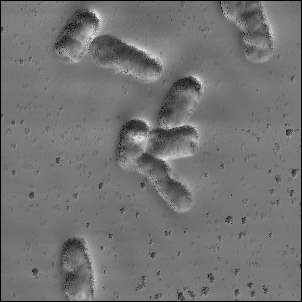
\includegraphics[keepaspectratio, width=\linewidth]{images/ec_o2a.png}
			\caption{Originale}
		\end{subfigure}
		\hspace{10pt}
		\begin{subfigure}{0.4\linewidth}
			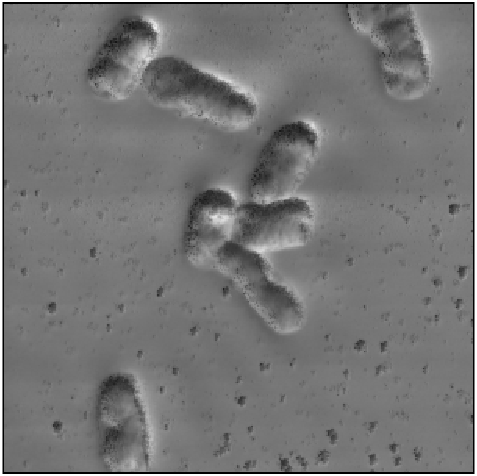
\includegraphics[keepaspectratio, width=\linewidth]{images/gauss_05.png}
			\caption{$\sigma = 0.5$}
		\end{subfigure}\\[4pt]
		\begin{subfigure}{0.4\linewidth}
			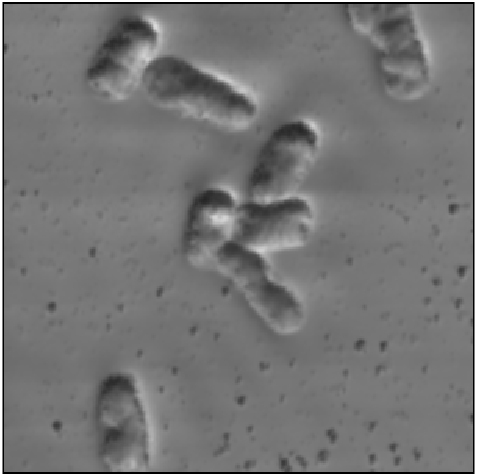
\includegraphics[keepaspectratio, width=\linewidth]{images/gauss_1.png}
			\caption{$\sigma = 1$}
		\end{subfigure}
		\hspace{10pt}
		\begin{subfigure}{0.4\linewidth}
			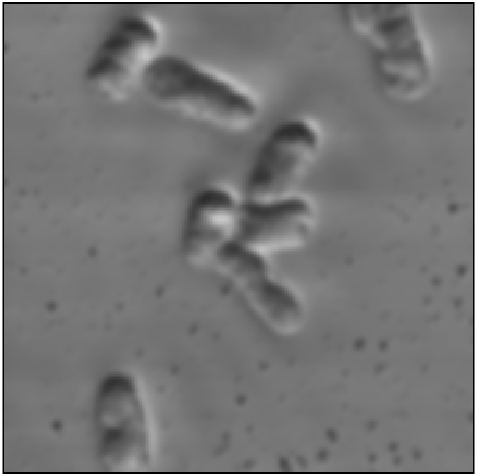
\includegraphics[keepaspectratio, width=\linewidth]{images/gauss_2.png}
			\caption{$\sigma = 2$}
		\end{subfigure}
		\caption{Effetto del parametro $\sigma$ sul filtraggio}
	\end{figure}

	\item La funzione gaussiana è separabile. Questa proprietà è importante per la complessità computazionale di questo filtro, in quanto si può applicare una funzione gaussiana 1D in una direzione e poi nell'altra, riducendo la complessità da $O(N^2)$ a $O(2N)$.
	\begin{equation}
		e^{-\frac{x^2+y^2}{2\sigma^2}}=e^{-\frac{x^2}{2\sigma^2}}e^{-\frac{y^2}{2\sigma^2}}
	\end{equation}
	\item Lo spettro della trasformata di Fourier della funzione gaussiana è esso stesso una funzione gaussiana. Questa proprietà può essere di aiuto per ridurre dei segnali ad alta frequenza dalle immagini e mantenere segnali più utili.
	\begin{equation}
		\hat{G}[u,v] = \hat{G_1}[u]\cdot\hat{G_1}[v] = \sum_{n=0}^{N-1}G[n]e^{-2\pi i\frac{nu}{N}}\cdot\sum_{m=0}^{M-1}G[m]e^{-2\pi i\frac{mv}{M}}
	\end{equation}
\end{enumerate}

\subsection{Filtro box}

Il \textbf{filtro box} è un filtro lineare costante nel dominio spaziale in cui ogni pixel dell'immagine viene sostituito con la media aritmetica dei valori dei pixel nel suo intorno di raggio $r$. Grazie al \textit{Teorema di Lindeberg-Lévy}, una ripetuta applicazione di questo filtro può essere usata per approssimare un filtro gaussiano.\cite{getreuer_2013}

\begin{equation}
	\operatorname{box}[i,j] = \frac{1}{(2r+1)^2}\sum_{n=-r}^{r}\sum_{m=-r}^{r} I(x+n, y+m)
\end{equation}
\\[-10pt]
Utilizzando dei pesi uguali per tutti gli elementi dell'intorno, può essere implementato utilizzando un algoritmo di accumulo molto più semplice, che è nettamente più veloce rispetto all'utilizzo di un algoritmo di finestra mobile, passando da una complessità temporale di $O(m^2n^2)$ ad una di $O(m^2)$, dove $m$ è la grandezza dell'immagine e $n$ è la grandezza della finestra.\cite{jarosz_2001}

Questo filtro, a differenza del filtro gaussiano, non può essere utilizzato efficacemente nel dominio delle frequenze in quanto si trasforma in un seno cardinale ed ha supporto spaziale infinito. Dovendo essere limitato in banda per essere utilizzato, può provocare degli artefatti di ringing nelle regioni in cui il valore del segnale cambia repentinamente. Questo comportamento prende il nome di \textit{fenomeno di Gibbs}.\cite{carslaw_1925}\\

\begin{figure}[ht]
	\centering
	\begin{subfigure}{0.4\linewidth}
		\centering
		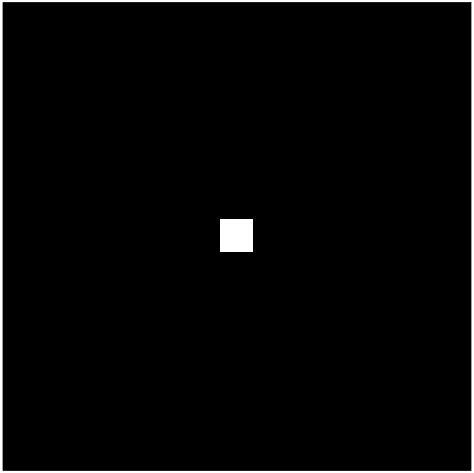
\includegraphics[keepaspectratio, width=\linewidth]{images/box_spatial.png}
		\caption{Filtro}
	\end{subfigure}
	\hspace{20pt}
	\begin{subfigure}{0.4\linewidth}
		\centering
		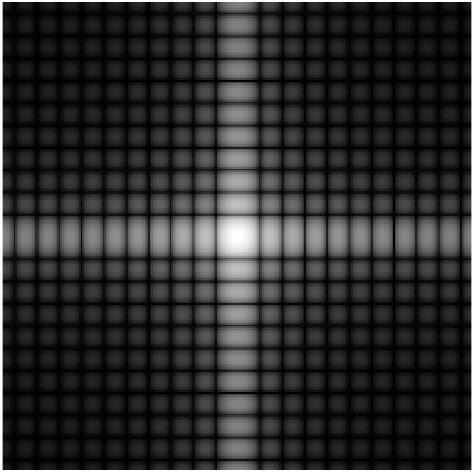
\includegraphics[keepaspectratio, width=\linewidth]{images/box_spectrum.png}
		\caption{Spettro}
	\end{subfigure}
	\caption{Esempio di filtro box}
\end{figure}

\begin{equation}
	\begin{aligned}
		\operatorname{box}(u,v) \quad\overset{\mathcal{F}}{\longrightarrow}\quad \hat{B}(x,y) &=  \frac{1}{a^2}\int_{-a/2}^{a/2}e^{2\pi iux}\,du\int_{-a/2}^{a/2}e^{2\pi ivy}\,dv =\\
		\boxed{a = 2r + 1} \qquad\quad &= \operatorname{sinc}(ax)\cdot\operatorname{sinc}(ay)
	\end{aligned}
\end{equation}

\begin{figure}[ht]
	\centering
	\begin{subfigure}{0.4\linewidth}
		\centering
		
\includegraphics[keepaspectratio, width=\linewidth]{images/ringing_orignal.png}
		\caption{Immagine originale}
	\end{subfigure}
	\hspace{20pt}
	\begin{subfigure}{0.4\linewidth}
		\centering
		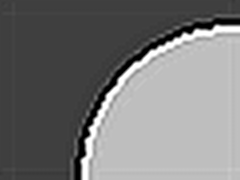
\includegraphics[keepaspectratio, width=\linewidth]{images/ringing_artifact.png}
		\caption{Immagine con artefatti}
	\end{subfigure}
	\caption[Artefatti di un filtro passa-basso ideale]{
		Artefatti di un filtro passa-basso \cite{ringingImage}}
\end{figure}

\subsection{Filtro mediana}

Il \textbf{filtro mediana} è un filtro simile al filtro box, con la differenza che ogni pixel dell'immagine è sostituito dalla mediana dei valori dei pixel nel suo intorno invece che la media, quindi non è un filtro lineare. Questo filtro è largamente usato nell'elaborazione delle immagini perché, sotto alcune condizioni, permette di rimuovere il rumore senza modificare i dettagli dell'immagine.\cite{rezaee_2021}

Per piccole quantità di rumore gaussiano, il filtro mediano si è dimostrato essere migliore del filtro gaussiano per rimuovere il rumore preservando i bordi per una determinata dimensione della finestra.\cite{castro_2009} Questo filtro è invece particolarmente efficace su rumori di tipo impulsivo, come il rumore \textit{salt \& pepper} e il rumore \textit{Schottky}.\cite{arce_2004}\\

\begin{figure}[ht]
	\centering
	\begin{subfigure}{0.4\linewidth}
		\centering
		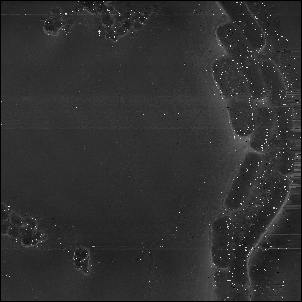
\includegraphics[keepaspectratio, width=\linewidth]{images/bs_o2p.png}
		\caption{Immagine originale}
	\end{subfigure}
	\hspace{20pt}
	\begin{subfigure}{0.4\linewidth}
		\centering
		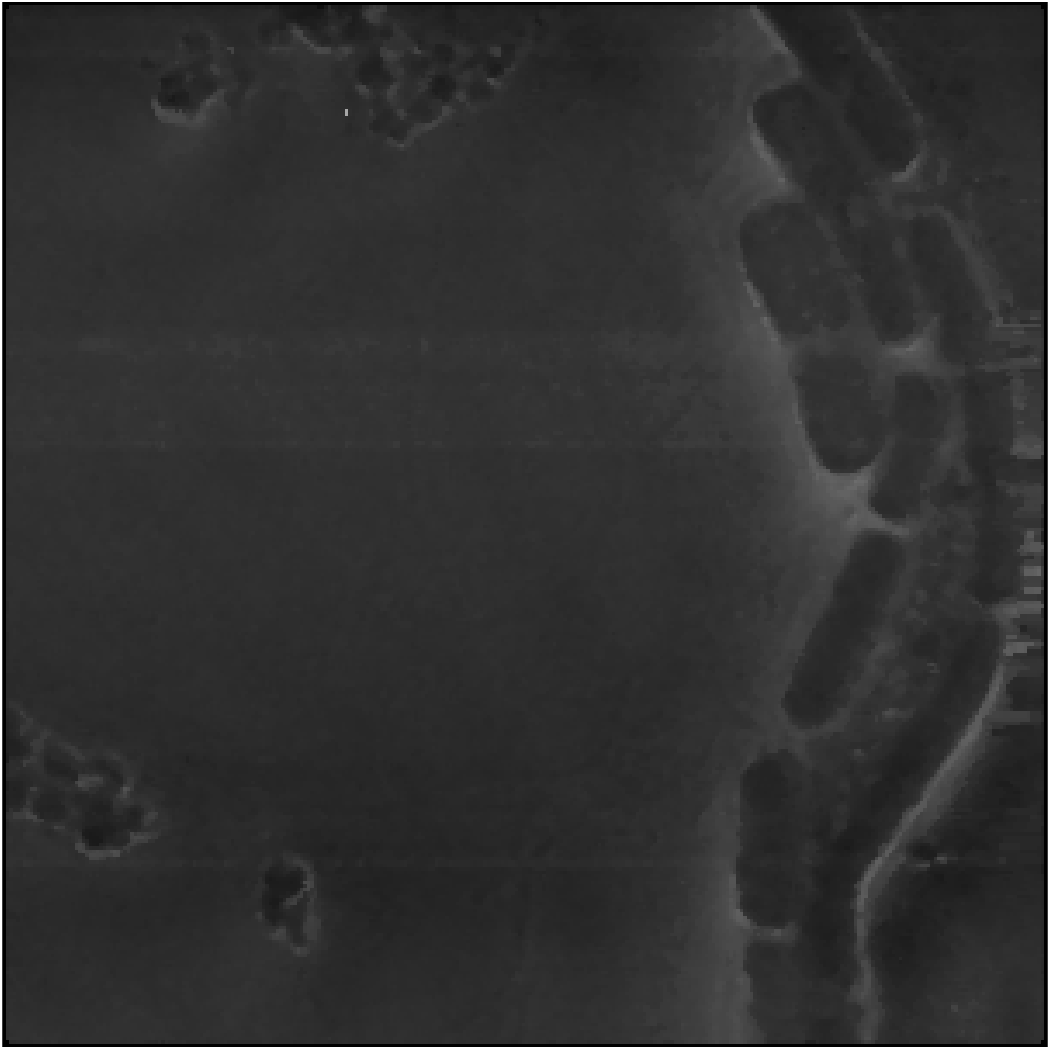
\includegraphics[keepaspectratio, width=\linewidth]{images/bs_o2p_medfilt.png}
		\caption{Immagine con filtro mediana $3\times3$}
	\end{subfigure}
	\caption[Immagine s-SNOM O2P di esemplari di \textit{Bacillus subtilis}]{
		Immagine \acrshort{ssnom} O2P di esemplari di \textit{Bacillus subtilis}}
\end{figure}

\subsection{Filtro Wiener}

Il \textbf{filtro Wiener} è un filtro originariamente ideato per calcolare una stima statistica di un segnale sconosciuto usando un segnale correlato come input, di cui si conosce la componente di rumore, e filtrarlo per produrre la stima. Questo filtro, ideato da \textit{Norbert Wiener} nel 1942,\cite{wiener_1942} ha l'obiettivo di  minimizzare l'errore quadratico medio (\acrshort{mse}) tra il processo stocastico stimato e il processo desiderato.\cite{oppenheimer_2010}

Per usare questo filtro, l'immagine e il suo rumore vengono considerati come variabili aleatorie. L'obiettivo è trovare una stima dell'immagine non corrotta $\hat{f}$ tale che l'errore quadratico medio tra di esse sia minimizzato. Questo filtro viene spesso usato anche per rimuovere una sfocatura di movimento tramite deconvoluzione. 

\begin{equation}
	\text{MSE} = \mathbb{E}\left[\left(f-\hat{f}\right)^2\right]
\end{equation}
\\[-10pt]
Per fare ciò bisogna rispettare dei presupposti: \cite{bergamasco_2016}

\begin{itemize}
	\itemsep0em
	\item Il rumore e l'immagine non devono essere correlati.
	\item Il rumore o l'immagine deve essere centrato, cioè a media nulla.
	\item I livelli di intensità nella stima sono una funzione lineare dei livelli nell'immagine degradata.
\end{itemize}
\begin{align}
	\hat{F}(u,v) &= \left[\frac{1}{H(u,v)}\cdot\frac{\left|H(u,v)\right|^2}{\left|H(u,v)\right|^2+S_\eta(u,v)/S_f(u,v)}\right]G(u,v)\\[5pt]
	H(u,v) &= \text{Funzione di degradazione} \nonumber \\
	\left|H(u,v)\right|^2 &= \text{Spettro di potenza di } H \nonumber \\
	S_\eta(u,v) &= \text{Spettro di potenza del rumore} \nonumber \\
	S_f(u,v) &= \text{Spettro di potenza dell'immagine non degradata} \nonumber 
\end{align}

Se il rumore è bianco allora il suo spettro di potenza sarà costante per tutto il dominio. Usando un'approssimazione ragionevole di $S_f(u,v)$ è possibile sostituire il rapporto con un termine costante.

\begin{equation}
	\hat{F}(u,v)= \left[\frac{1}{H(u,v)} \cdot \frac{\left|H(u,v)\right|^2}{\left|H(u,v)\right|^2+k}\right] G(u,v)
\end{equation}

\subsection{Filtro bilaterale}

Il \textbf{filtro bilaterale} smussa le immagini preservando i bordi allo stesso tempo per mezzo di una combinazione non lineare di valori nell'intorno del pixel. Questo filtro combina l'intensità dei pixel sia in base alla loro vicinanza geometrica che alla loro similarità fotometrica e preferisce valori vicini tra loro rispetto a valori distanti sia nel dominio che nel codominio.\cite{tomasi_1998}

\begin{equation}
	I_f(x) = \frac{1}{k(x)}\iint_{-\infty}^{\infty}I(x)c(\xi,x)s(f(\xi),f(x))\,d\xi
\end{equation}
\\[-10pt]
La funzione $s(f(\xi),f(x))$ misura la similarità fotometrica tra il punto $x$ al centro dell'intorno e il punto vicino $\xi$, mentre la funzione $c(\xi,x)$ ne misura la vicinanza geometrica. La funzione $k(x)$ definisce il fattore di normalizzazione.

\begin{equation}
	k(x) = \iint_{-\infty}^{\infty}c(\xi,x)s(f(\xi),f(x))\,d\xi
\end{equation}
\\[-10pt]
Un caso importante del filtro bilaterale è quello in cui sia la funzione di vicinanza che la funzione di similarità sono funzioni gaussiane della distanza euclidea tra i loro argomenti.
\begin{align}
	c(\xi,x) &= \exp\left(-\frac{||\xi-x||^2}{2\sigma^2_d}\right)\\
	s(\xi,x) &= \exp\left(-\frac{||f(\xi)-f(x)||^2}{2\sigma^2_r}\right)
\end{align}

La diffusione geometrica $\sigma_d$ nel dominio viene scelta in base alla quantità di filtraggio passa-basso desiderata. Allo stesso modo, la diffusione fotometrica $\sigma_r$ nel codominio dell'immagine viene impostata per ottenere la quantità di combinazione desiderata delle intensità dei pixel.

Questo filtro è anche usato per il filtraggio di immagini a colori in quanto consente di combinare opportunamente le tre bande di colore e di misurare le distanze fotometriche tra i pixel nello spazio combinato. Inoltre, questa distanza combinata può essere fatta corrispondere in modo preciso alla dissimilarità percepita dal sistema visivo umano (\acrlong{hvs} --- \acrshort{hvs}) utilizzando la distanza euclidea nello spazio colore CIE-Lab.\cite{wyszecki_2000}

\subsection{Filtro guidato}

Il \textbf{filtro guidato} genera l'immagine di uscita prendendo in considerazione il contenuto spaziale di un'altra immagine, detta di guida, che può essere l'immagine di input stessa o un'altra immagine diversa. Questo filtro ha la proprietà di preservare i bordi come il filtro bilaterale, ma non soffre degli stessi artefatti di inversione del gradiente.\cite{durand_2002}
\begin{equation}
	f[i] = \sum_{j}I[j]W\{G\}[i,j]
\end{equation}

L'uscita del filtro è una media pesata in cui il kernel di filtraggio $W\{G\}$ è funzione dell'immagine guida $G$ ed è indipendente dall'immagine da filtrare $I$, mentre $i$ e $j$ sono le coordinate di due pixel. Un esempio concreto di questo kernel è il filtro bilaterale congiunto, che si comporta come un filtro bilaterale quando $G$ e $I$ sono identiche.\cite{petschnigg_2004}
\begin{equation}
	W^{bf}\{G\}[i,j] = \frac{1}{K} \exp\left(-\frac{|i-j|^2}{\sigma^2_r}\right) \exp\left(-\frac{|G[i]-G[j]|^2}{\sigma_r^2}\right)
\end{equation} 

Il presupposto fondamentale del filtro guidato è un modello lineare locale tra la guida $G$ e l'uscita del filtro $f$. Assumendo che $f$ sia una trasformazione lineare di $G$ in un intorno $\omega_k$ centrato sul pixel $k$, è sicuro che $f$ presenta un bordo solo se è presente anche in $G$, poiché $\nabla f = a\nabla G$.\cite{he_2013}
\begin{equation}
	f[i] = a_kG[i]+b_k,\ \forall i\in\omega_k
\end{equation}

Per determinare i coefficienti lineari, bisogna cercare una soluzione che minimizzi la differenza tra l'immagine in ingresso $I$ e in uscita $f$. La soluzione può essere espressa come una regressione lineare.
\begin{align}
	a_k &= \frac{\frac{1}{|\omega|}\sum_{i\in\omega_k}G[i]I[i]-\mu_k\bar{I}_k}{\sigma_k^2+\epsilon}\\
	b_k &= \bar{I}_k-a_k\mu_k
\end{align}

Dopo aver applicato questo modello a tutti gli intorni dell'immagine, può essere calcolato il peso del filtro facendo la media tra tutti gli intorni che includono un certo pixel $i$.

\begin{equation}
	W\{G\}[i,j] = \frac{1}{|\omega|^2} \sum_{(i,j)\in\omega_k} \left[1+\frac{(G[i]-\mu_k)(G[j]-\mu_k)}{\sigma_k^2+\epsilon}\right]
\end{equation}

\begin{figure}[ht]
	\centering
	\begin{subfigure}{0.32\linewidth}
		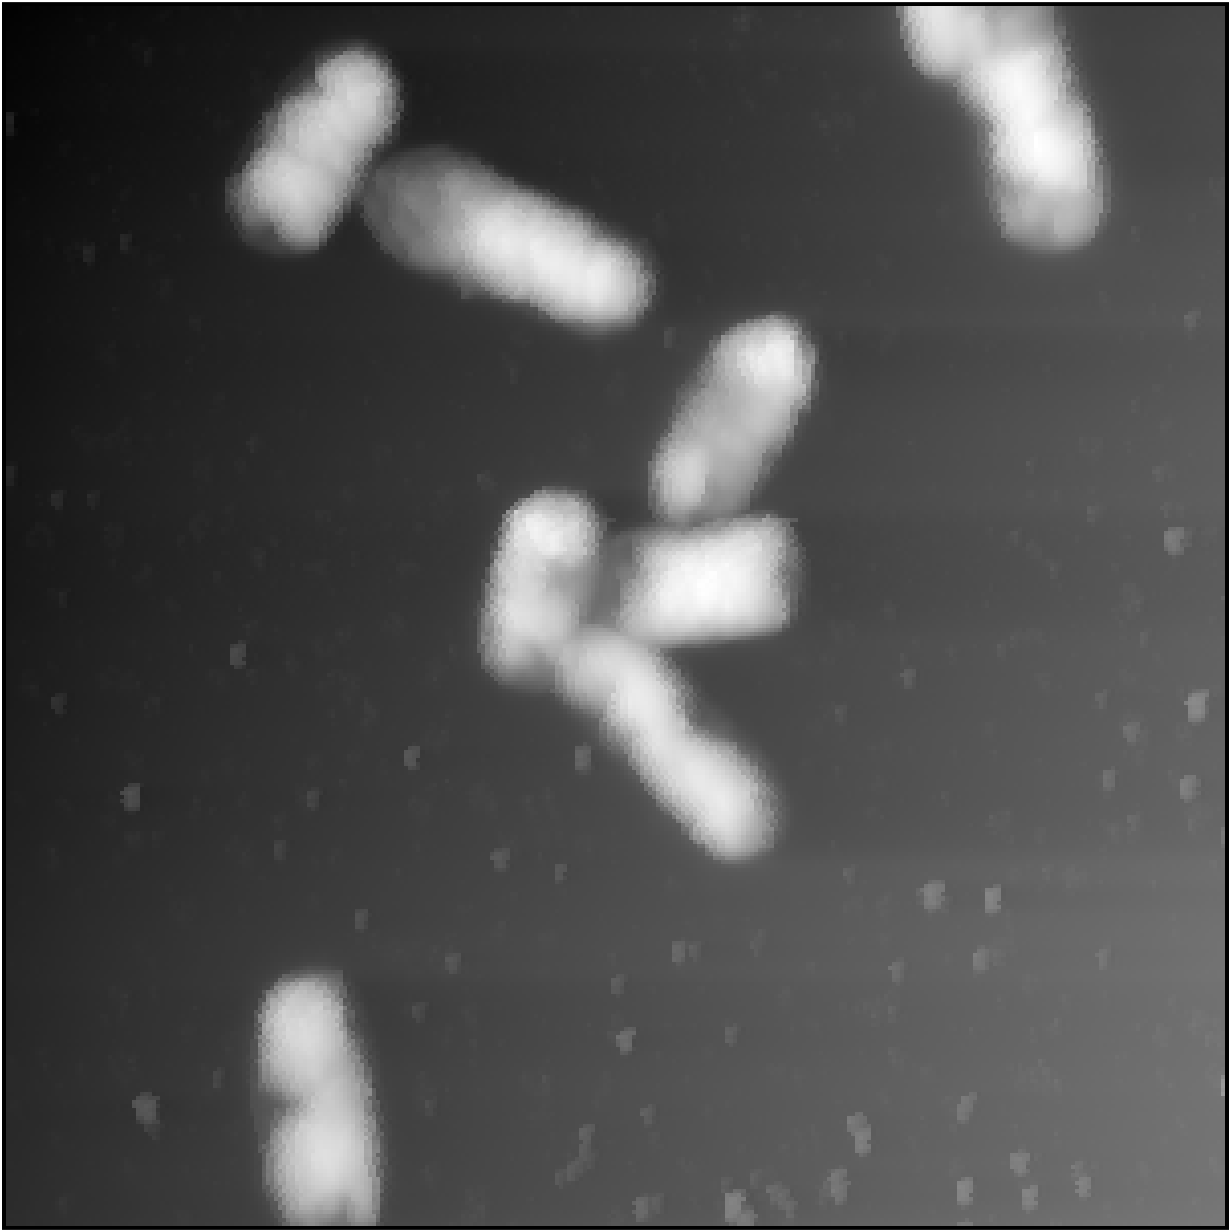
\includegraphics[keepaspectratio, width=\linewidth]{images/entero_z.png}
		\caption{Topografia \acrshort{afm}}
	\end{subfigure}
	\begin{subfigure}{0.32\linewidth}
		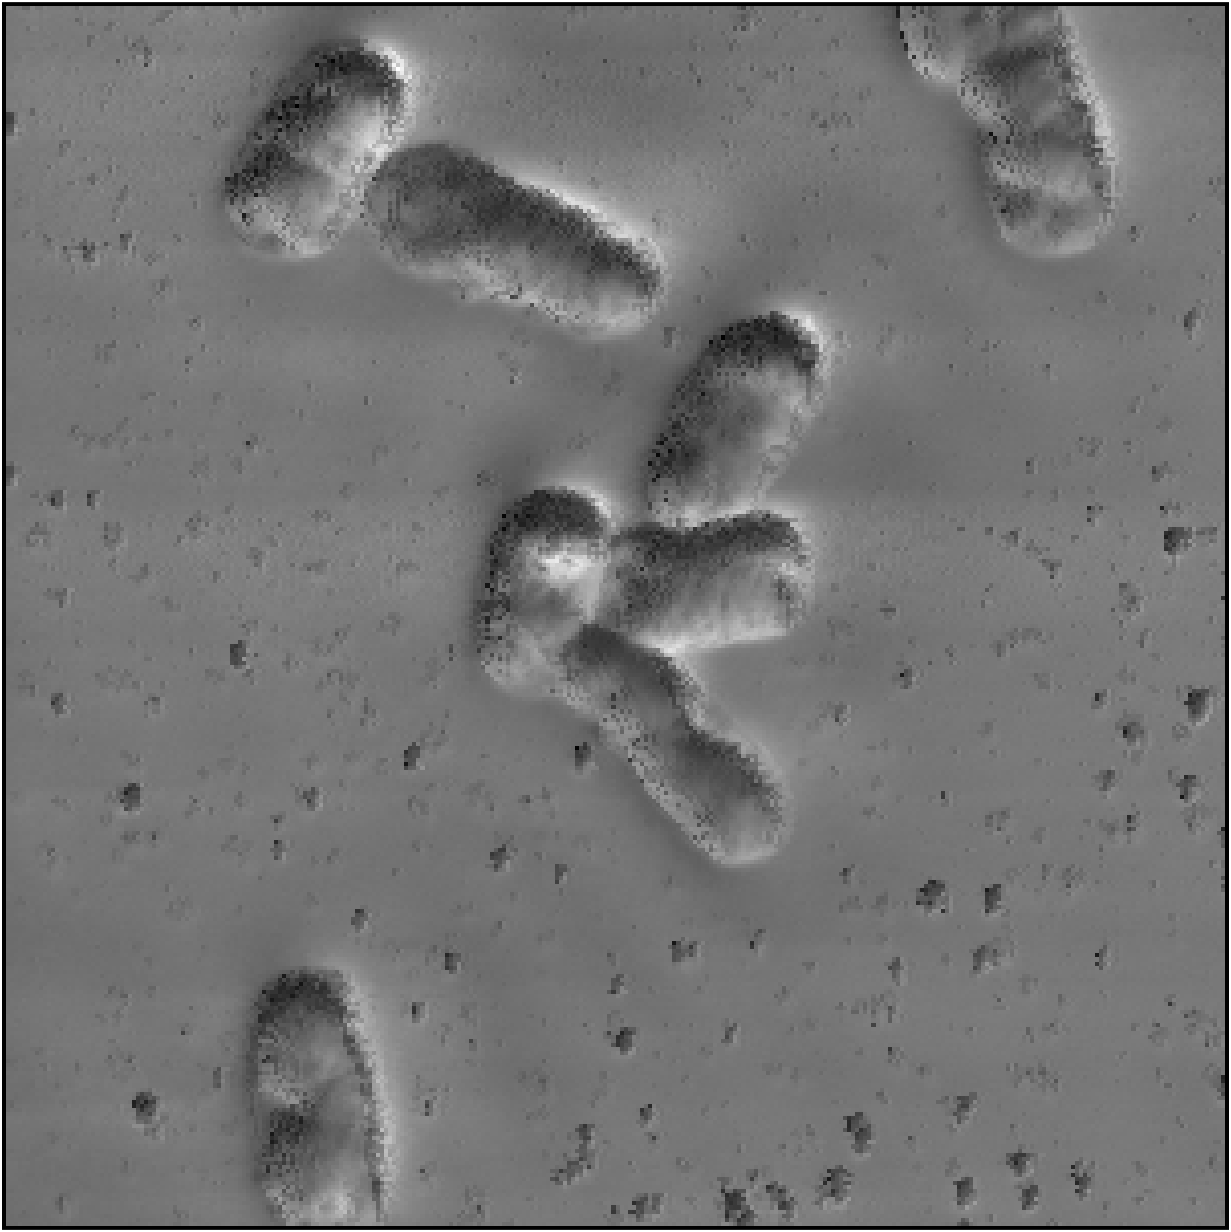
\includegraphics[keepaspectratio, width=\linewidth]{images/entero_o2a.png}
		\caption{\acrshort{ssnom} O2A}
	\end{subfigure}
	\begin{subfigure}{0.32\linewidth}
		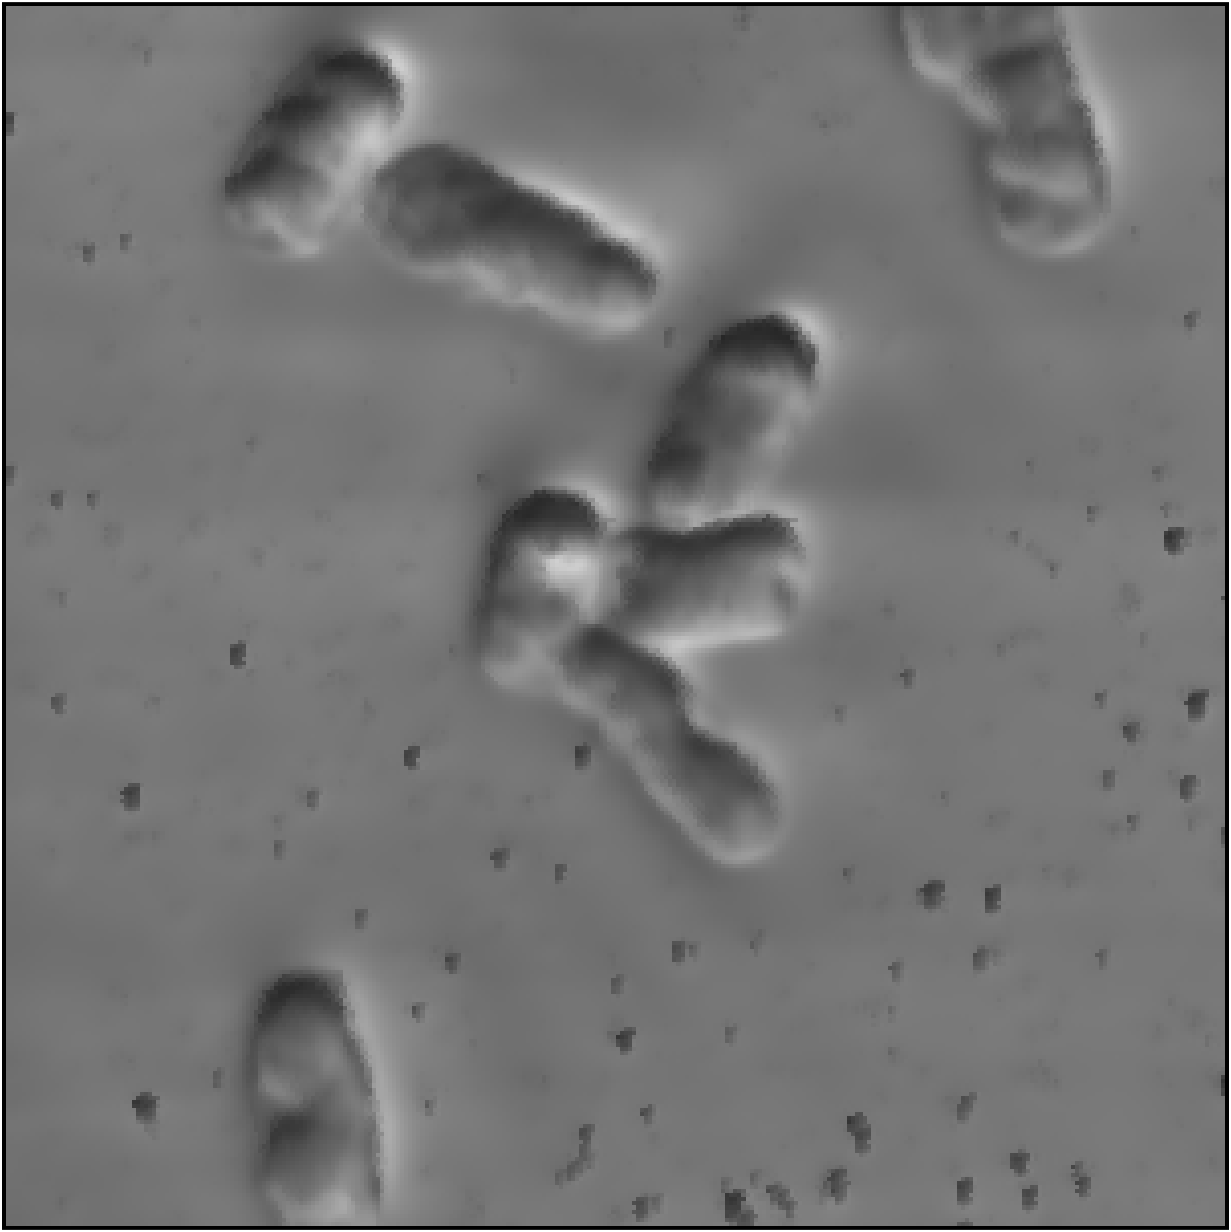
\includegraphics[keepaspectratio, width=\linewidth]{images/entero_guided.png}
		\caption{Immagine filtrata}
	\end{subfigure}
	\caption[Filtro guidato dall'immagine di topografia AFM]{
		Filtro guidato dall'immagine di topografia \acrshort{afm}}
\end{figure}

\subsection{Filtro a media non locale}

Il \textbf{filtro a media non locale} (NLM), a differenza dei filtri locali come il filtro gaussiano, non determina il valore di un pixel basandosi sulle caratteristiche del suo intorno ma utilizza una media dell'intera immagine, pesata in ogni punto in base alla similarità con il pixel in esame.\cite{buades_2011}

Data un'immagine rumorosa discreta $v = \left\{v(i) | i\in I\right\}$, il valore stimato dal filtro per il pixel $i$ è calcolato come una media pesata di tutti i pixel dell'immagine, dove la famiglia dei pesi $w(i,j)$ dipende dalla similarità tra le intensità degli intorni $\mathcal{N}_i$ e $\mathcal{N}_j$, rispettivamente dei pixel $i$ e $j$.
\begin{align}
	\text{NL}[v](i) &= \sum_{j\in I}w(i,j)v(j)\\
	w(i,j) &= \frac{1}{Z(i)}\exp\left(-\frac{\left\lVert v(\mathcal{N}_i) - v(\mathcal{N}_j) \right\lVert^2_{2,a}}{h^2}\right)\\
	Z(i) &= \sum_{j\in I}\exp\left(-\frac{\left\lVert v(\mathcal{N}_i) - v(\mathcal{N}_j) \right\lVert^2_{2,a}}{h^2}\right)
\end{align}

Questa similarità viene misurata come una funzione decrescente della distanza euclidea pesata, dove $a$ è la deviazione standard del kernel gaussiano. Il parametro $h$ agisce modificando il grado di filtraggio: controlla il decadimento della funzione esponenziale e quindi il decadimento dei pesi in funzione delle distanze euclidee.\cite{buades_2005}\\

\begin{figure}[ht]
	\centering
	\begin{subfigure}{0.32\linewidth}
		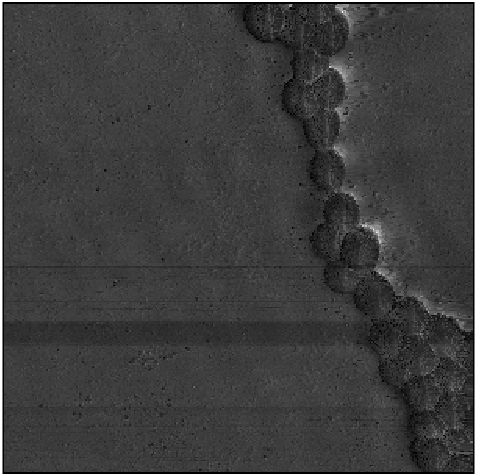
\includegraphics[keepaspectratio, width=\linewidth]{images/sa_o2a.png}
		\caption{Originale}
	\end{subfigure}
	\begin{subfigure}{0.32\linewidth}
		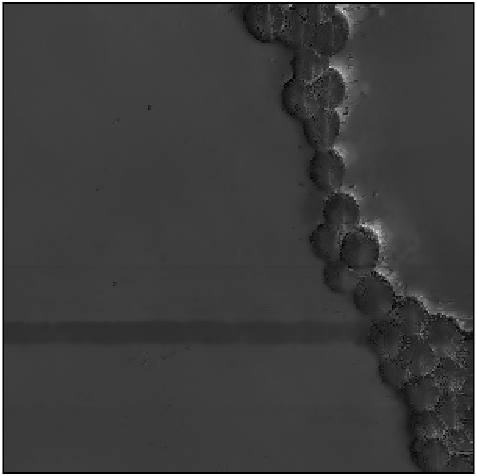
\includegraphics[keepaspectratio, width=\linewidth]{images/nlm_0025.png}
		\caption{$h = 0.025$}
	\end{subfigure}
	\begin{subfigure}{0.32\linewidth}
		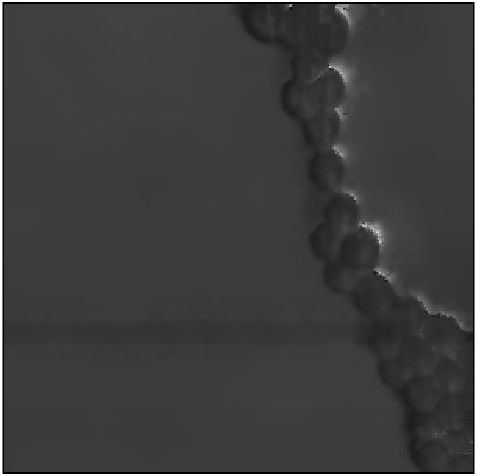
\includegraphics[keepaspectratio, width=\linewidth]{images/nlm_005.png}
		\caption{$h = 0.05$}
	\end{subfigure}
	\caption{Effetto del parametro $h$ sul filtraggio}
\end{figure}

Il filtro NLM non confronta solo le intensità dei singoli pixel, ma anche la configurazione geometrica dell'intero intorno. Questo consente un confronto più robusto rispetto ai filtri locali.

\begin{figure}[ht]
	\centering
	\begin{subfigure}{0.32\linewidth}
		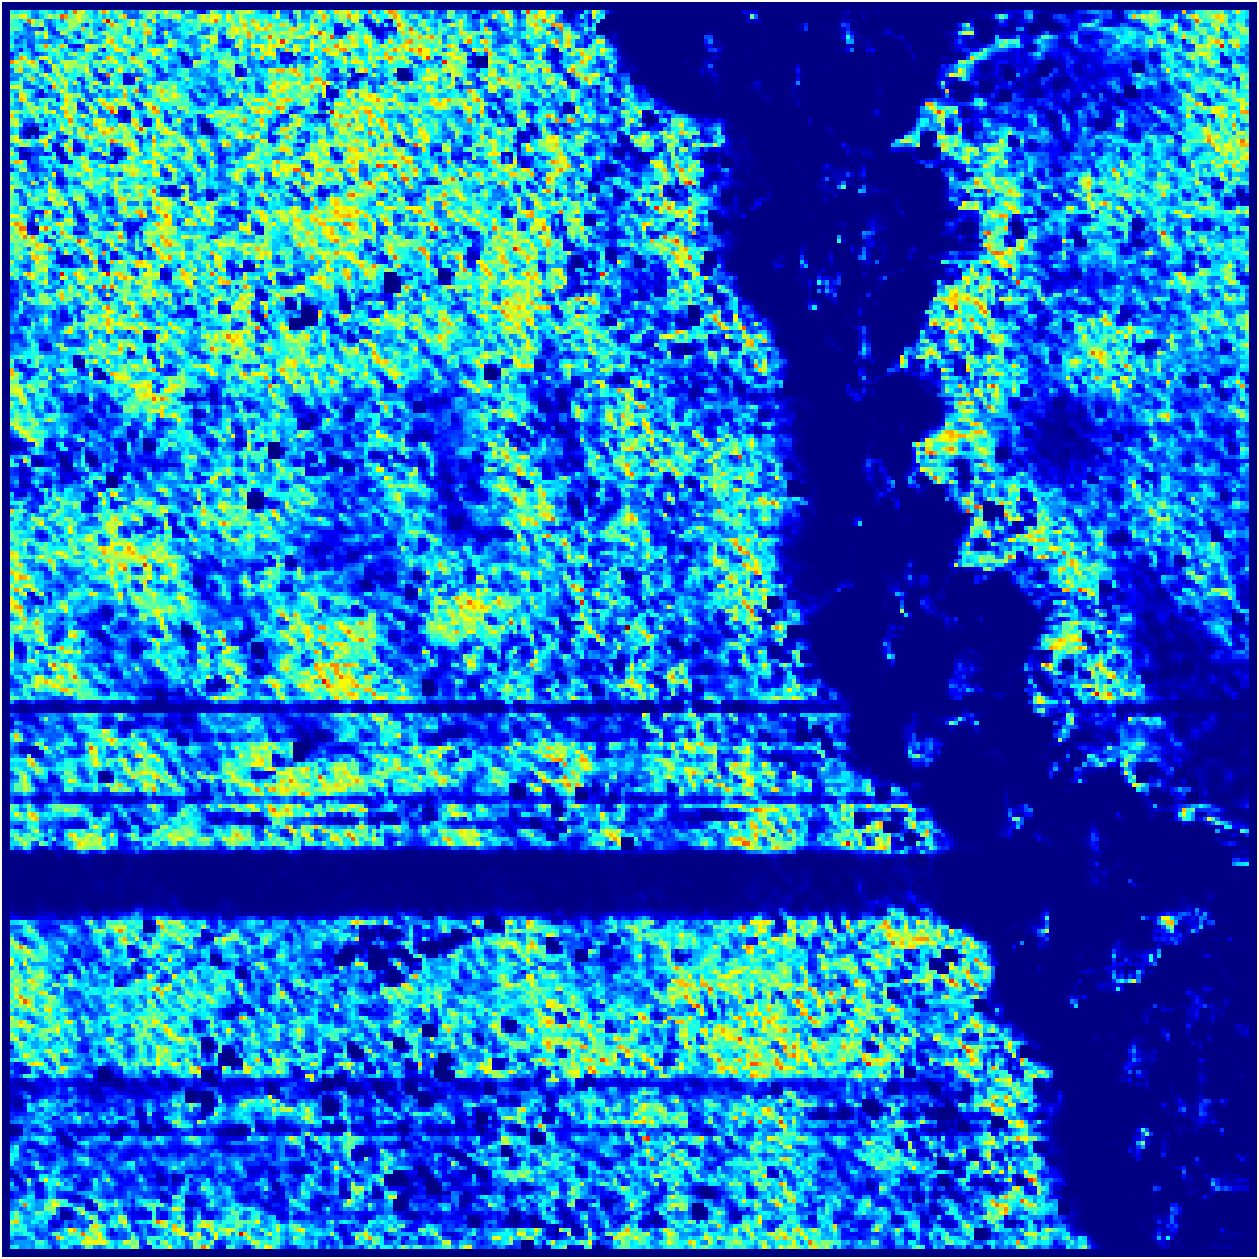
\includegraphics[keepaspectratio, width=\linewidth]{images/nlm_weights_3.png}
		\caption{$3\times3$}
	\end{subfigure}
	\begin{subfigure}{0.32\linewidth}
		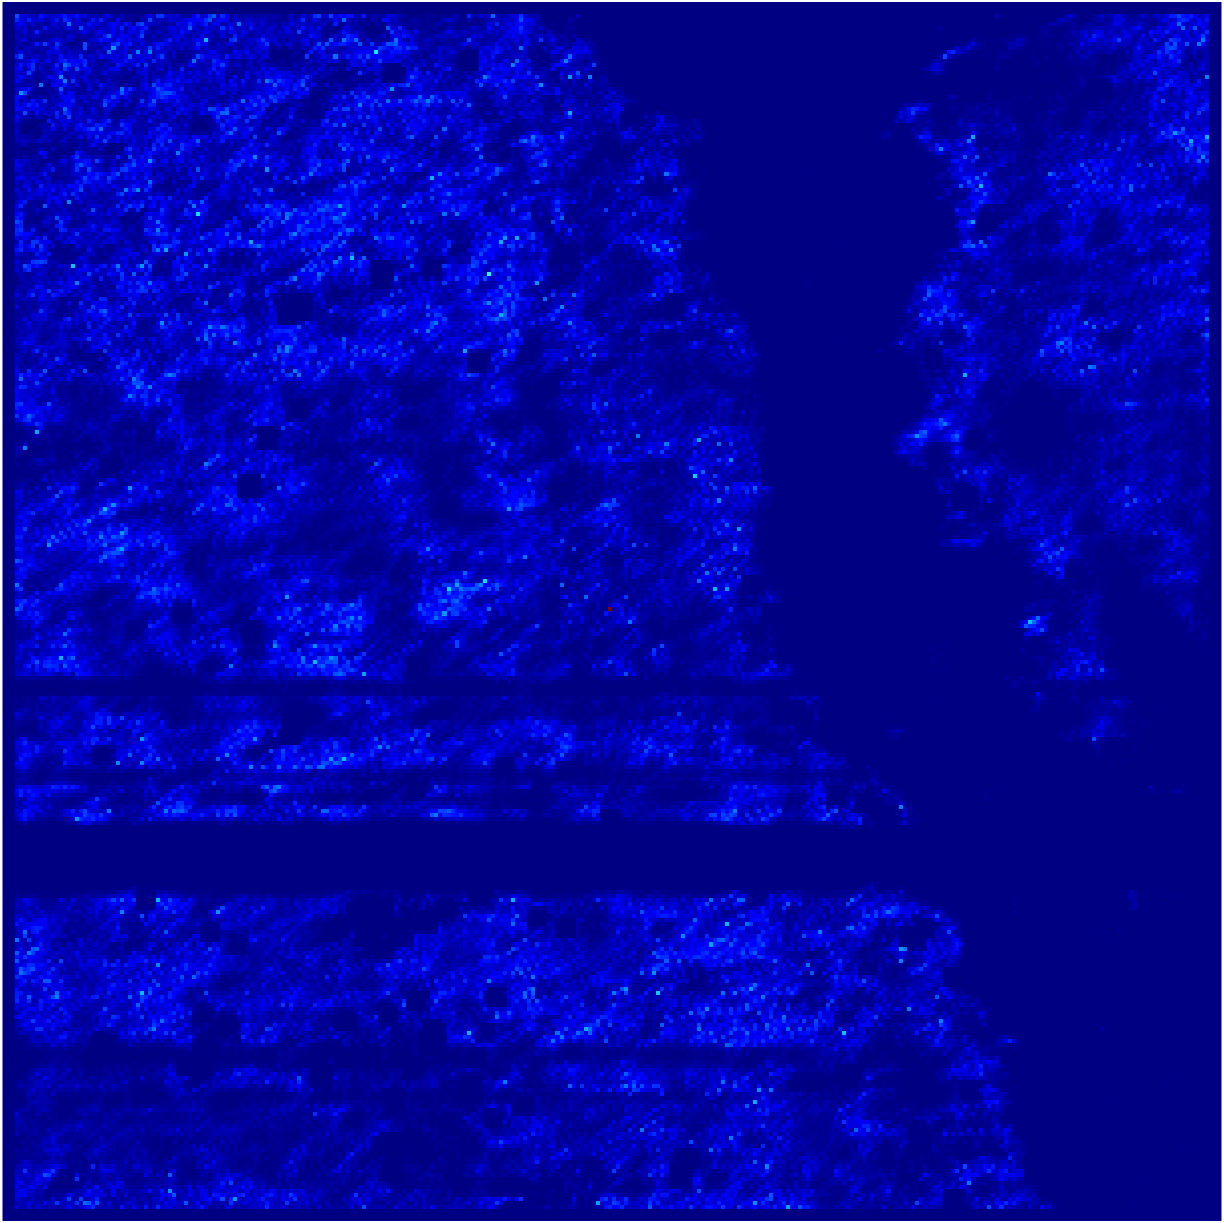
\includegraphics[keepaspectratio, width=\linewidth]{images/nlm_weights_5.png}
		\caption{$5\times5$}
	\end{subfigure}
	\begin{subfigure}{0.32\linewidth}
		\begin{tikzpicture}
			\begin{scope}[
				node distance = 11mm,
				inner sep = 0pt,spy using outlines={rectangle, red, magnification=6}]
				\node (n0)  {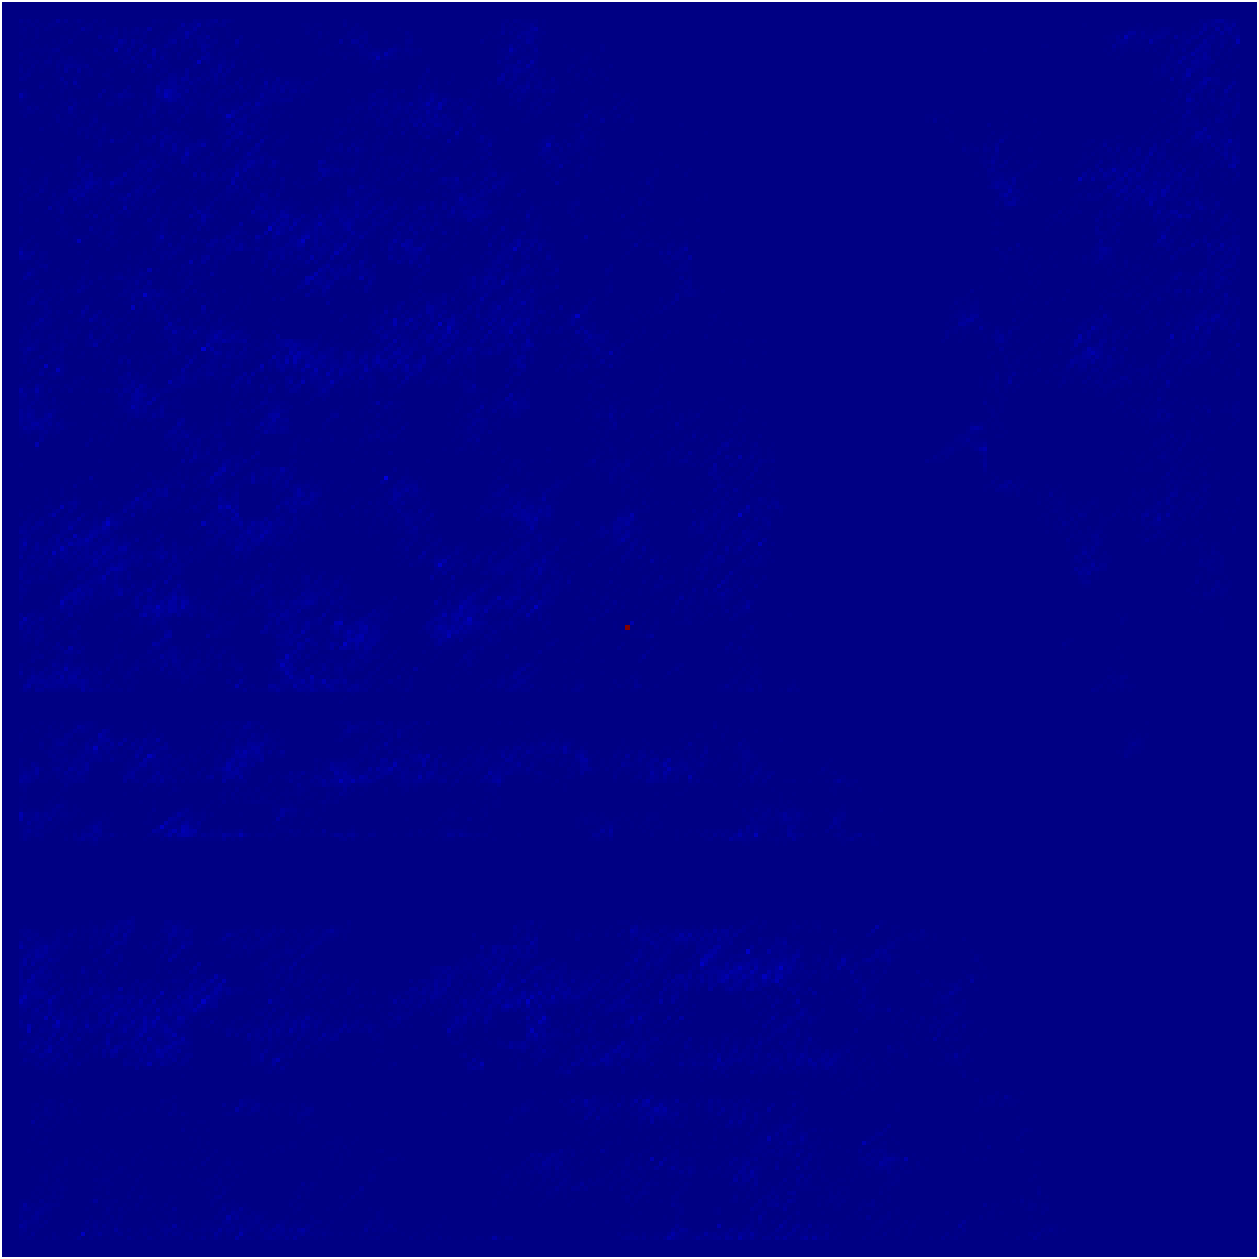
\includegraphics[keepaspectratio, width=\textwidth]{images/nlm_weights_7.png}};
				
				\spy [white,size=1cm] on (n0.center) in node[below right=of n0.north west];
			\end{scope}
			\draw[dashed,white] (tikzspyonnode.north east) -- (tikzspyinnode.north east);
			\draw[dashed,white] (tikzspyonnode.south west) -- (tikzspyinnode.south west);
		\end{tikzpicture}
		\caption{$7\times7$}
	\end{subfigure}
	\caption[Distribuzione dei pesi rispetto al	pixel centrale dell'immagine]{\begin{tabular}[t]{@{}l@{}}
			Effetto della grandezza dell'intorno sulla distribuzione dei pesi rispetto al\\
			pixel centrale dell'immagine
		\end{tabular}}
\end{figure}

\subsection{Filtro BM3D}

Il \textbf{filtro BM3D} (Block-Matching and 3D Filtering) è un'estensione del filtro a media non locale che fa uso di una migliore rappresentazione sparsa nel dominio di trasformazione.\cite{manjon_2008}

Il primo passo consiste nel suddividere l’immagine in blocchi (patch) di dimensioni fisse e poi raggruppare insieme i blocchi simili da un algoritmo di block-matching, formando un tensore tridimensionale (gruppo) in cui ogni strato del volume è un blocco simile. Questi blocchi non sono necessariamente disgiunti ma possono anche sovrapporsi parzialmente.

Una volta raccolti i blocchi simili, è possibile applicare delle funzioni di trasformazione (come DCT o wavelet) per rappresentare questi gruppi in modo più compatto. Nello spazio trasformato, il rumore appare come elementi sparsi, mentre i dati reali (cioè i dettagli coerenti tra i blocchi) si concentrano in poche componenti. Si può quindi applicare un filtro sulla trasformata, come un filtro Wiener, per ridurre il rumore, eliminando i coefficienti minori.\cite{maggioni_2013}

Dopo il filtraggio, il tensore viene ricostruito tramite la trasformata inversa e i blocchi ripuliti vengono reinseriti nell’immagine. Dato che un pixel può comparire in più blocchi, l’immagine finale si ottiene come media pesata di tutti i contributi.\cite{dabov_2007}

\section{Metodi di valutazione}

Per misurare l'efficacia di questi filtri sono stati presi in considerazione diversi metodi di valutazione. La mancanza di immagini senza rumore di riferimento impedisce l'uso di metodi di valutazione full-reference (\acrshort{friqa}) ampiamente utilizzati, come \acrshort{psnr}\cite{korhonen_2012}, \acrshort{ssim}\cite{wang_2004} e \acrshort{cnr}.\cite{rodriguez_2018} La difficoltà nel valutare la qualità di queste immagini deriva anche dalla mancanza di valutazioni soggettive di esperti nel campo e dalla limitata quantità di letteratura su questo argomento.

In questo lavoro sono stati usati alcuni sistemi di valutazione cieca (\acrshort{nriqa}) basati su modelli statistici di immagini naturali, come \acrshort{brisque}\cite{mittal_2011}, \acrshort{niqe}\cite{mittal_2013} e \acrshort{piqe}\cite{venkatanath_2015}, usando i loro modelli predefiniti. Questi sistemi valutano la qualità dell'immagine con un punteggio da 0 in su, dove 0 corrisponde alla massima qualità. Oltre ai punteggi di questi modelli è stata misurata anche la variazione totale dell'immagine (\acrshort{tv}).

È stata inoltre condotta un'analisi correlativa tra le proprietà delle immagini di ampiezza \acrshort{snom} prese in esame e le corrispettive immagini di topografia \acrshort{afm}, in quanto questa immagine contiene una quantità di rumore molto inferiore rispetto alla prima.

\begin{figure}[ht]
	\centering
	\begin{subfigure}{0.4\linewidth}
		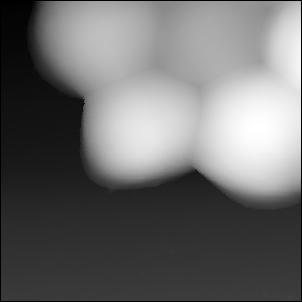
\includegraphics[keepaspectratio, width=\linewidth]{images/sa_zoom_z.png}
		\caption{Topografia \acrshort{afm}}
	\end{subfigure}\hspace{12pt}
	\begin{subfigure}{0.4425\linewidth}
		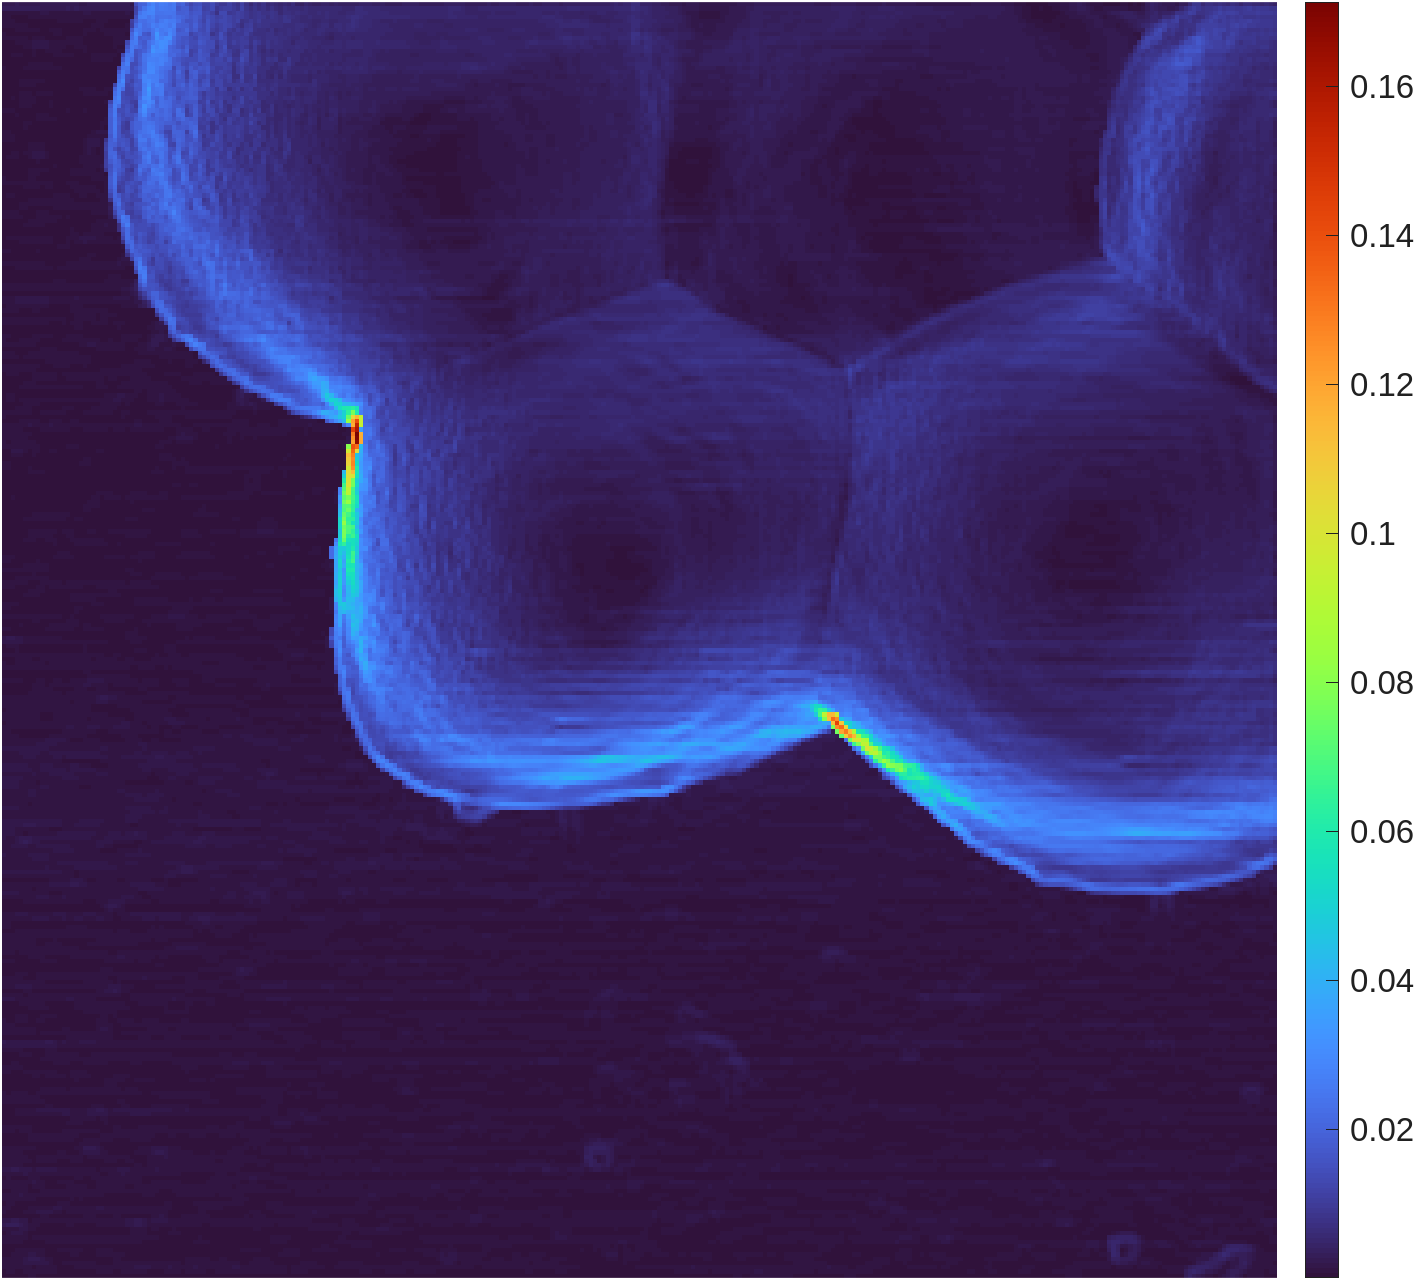
\includegraphics[keepaspectratio, width=\linewidth]{images/local_std_z.png}
		\caption{Deviazione standard topografia}
	\end{subfigure}\\[4pt]
	\begin{subfigure}{0.4\linewidth}
		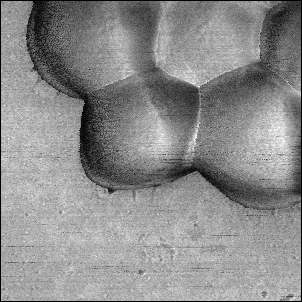
\includegraphics[keepaspectratio, width=\linewidth]{images/sa_zoom_o3a.png}
		\caption{Ampiezza \acrshort{ssnom} --- $3^a$ armonica}
	\end{subfigure}\hspace{12pt}
	\begin{subfigure}{0.4425\linewidth}
		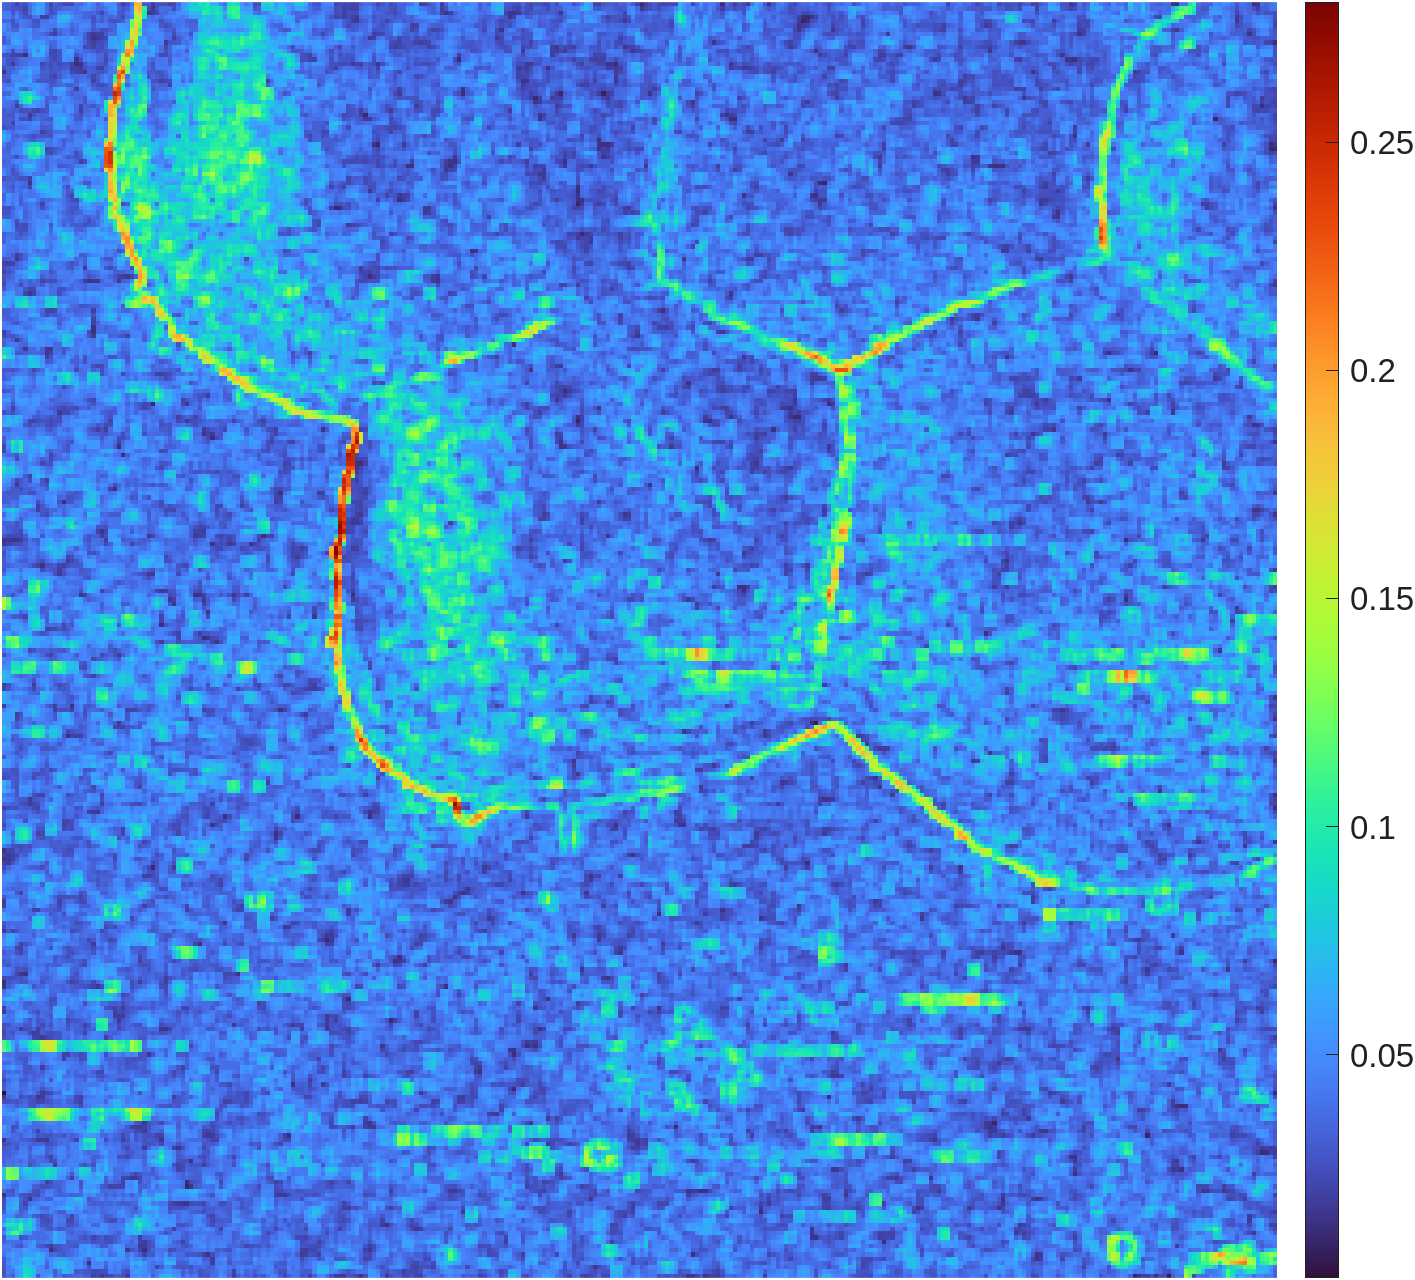
\includegraphics[keepaspectratio, width=\linewidth]{images/local_std_o3a.png}
		\caption{Deviazione standard ampiezza \acrshort{ssnom}}
	\end{subfigure}
	\caption[Confronto della deviazione standard locale tra immagini AFM e SNOM]{
		Confronto della deviazione standard locale tra immagini \acrshort{afm} e \acrshort{snom}}
\end{figure}

\subsection{Analisi correlativa}

Le immagini di topografia \acrshort{afm} e ampiezza \acrshort{snom}, anche se condividono delle informazioni spaziali correlate, non possono essere esaminate con i metodi di valutazione full-reference tradizionali poiché non rappresentano lo stesso contenuto. Le prime sono una mappa altimetrica del campione, mentre le seconde catturano le interazioni ottiche nel campo vicino, che dipendono dai materiali del campione.

Per svolgere questa analisi sono stati presi in considerazione cinque parametri:

\begin{enumerate}
	\itemsep0em
	\item Indice di Dice sui bordi
	\item Mutua informazione delle immagini
	\item Errore quadratico medio dell'entropia
	\item Congruenza di fase
	\item Modulo dei gradienti
\end{enumerate}

L'\textbf{indice di Dice} è usato per misurare la somiglianza tra due campioni studiando la presenza o assenza di elementi in comune, in questo caso la sovrapposizione tra l'immagine dei bordi della topografia e dell'ampiezza \acrshort{snom}. Un valore vicino a $1$ indica un'ottima sovrapposizione dei bordi mentre uno vicino a $0$ indica una scarsa sovrapposizione.\cite{carass_2020}

\begin{equation}
	S = 2\cdot \frac{\left|E_{X} \cap  E_{Y}\right|}{\left|E_{X}\right| + \left|E_{Y}\right|}
\end{equation}

La \textbf{mutua informazione} (\acrshort{mi}) è una misura statistica che quantifica quante informazioni una variabile contiene su un'altra, in questo caso un'immagine.\cite{shannon_1948} Questa misura è strettamente collegata al concetto di entropia di una variabile ed è ampiamente utilizzata nella correlazione e registrazione di immagini multimodale in cui vengono confrontati due diversi tipi di immagini,\cite{viola_1997} ad esempio RM e TAC,\cite{mclaughlin_2004, veninga_2004} usata in questo caso su \acrshort{afm} e \acrshort{ssnom}. La mutua informazione è nulla se $X$ e $Y$ sono variabili indipendenti.
\begin{equation}
	\begin{aligned}
		I(X,Y)  &= \sum_{x\in X}\sum_{y\in Y} p(x,y) \log\left(\frac{p(x,y)}{p_1(x)p_2(y)}\right) =\\
		&= H(X) + H(Y) - H(X,Y)
	\end{aligned}
\end{equation}

L'\textbf{entropia} è una misura della complessità spaziale dell'immagine, per cui regioni con un'alta entropia presentano strutture fine, texture o bordi marcati mentre regioni con un'entropia bassa presentano superfici lisce o uniformi. Ricavando l'errore quadratico medio dell'entropia rispetto all'immagine di topografia si può stimare la differenza di dettagli o rumore tra le due. Se l'errore è piccolo allora le due immagini avranno complessità spaziale simile negli stessi punti, mentre se è alto le strutture locali saranno differenti.
\begin{equation}
	\text{MSE} = \frac{1}{N}\sum_{i\in\Omega}\left(H_1(i)-H_2(i)\right)^2
\end{equation}

Un'altra misura per la stima delle strutture locali è la \textbf{congruenza di fase} (\acrlong{pc} --- \acrshort{pc}), secondo la quale le caratteristiche sono percepite in punti in cui le componenti di Fourier sono massime in fase. La congruenza di fase fornisce un modello semplice ma biologicamente plausibile di come il sistema visivo umano rileva e identifica le caratteristiche di un'immagine.\cite{kovesi_1999,morrone_1988}

Nel caso di segnali unidimensionali, questi si possono scomporre in $N$ componenti armoniche con ampiezza locale $A_n(x)$ e fase locale $\phi_n(x)$. La congruenza di fase nella posizione $x$ sarà il massimo allineamento di queste fasi. Quando tutte le fasi sono allineate, i termini del coseno valgono $1$ e di conseguenza si avrà $\text{PC} = 1$, mentre quando sono casuali il numeratore tende a $0$.
\begin{align}
	\text{PC}(x) &= \underset{\bar{\phi}(x)}{\max}\frac{\sum_n A_n(x) \cos\left(\phi_n(x) - \bar{\phi}(x)\right)}{\sum_n A_n(x)}\\[10pt]
	\bar{\phi}(x) &= \tan^{-1}\left(\frac{\sum_n A_n(x)\sin\phi_n(x)}{\sum_n A_n(x)\cos\phi_n(x)}\right)
\end{align}

Questo metodo non può essere usato per segnali bidimensionali come le immagini perché la trasformata di Hilbert non è definita per spazi multidimensionali e la trasformata di Fourier non è adatta a localizzare spazialmente le informazioni in frequenza. I sistemi moderni utilizzano una banca di filtri log-Gabor in diverse scale spaziali $s$ e orientamenti $o$ per misurare la congruenza di fase. Questo è implementato con delle paia di filtri in quadratura, in cui uno è pari $M^e_{s,o}$ e l'altro è dispari $M^o_{s,o}$.\cite{kovesi_2003}
\begin{align}
	\text{PC}(\mathbf{x}) &= \frac{\sum_o \mathcal{E}_o(\mathbf{x}) - T_o}{\sum_o\sum_s A_{s,o}(\mathbf{x})+\varepsilon}\\[6pt]
	\mathcal{E}_o(\mathbf{x}) &= \sqrt{\left(\sum_s I(\mathbf{x}) * M^e_{s,o}\right)^2 + \left(\sum_s I(\mathbf{x}) * M^o_{s,o}\right)^2}\\[6pt]
	A_{s,o}(\mathbf{x}) &= \sqrt{\left(I(\mathbf{x}) * M^e_{s,o}\right)^2 + \left(I(\mathbf{x}) * M^o_{s,o}\right)^2}
\end{align}

la congruenza di fase è combinata con l'\textbf{ampiezza dei gradienti} per formare l'indice \acrshort{fsim}, usato per misurare la similarità strutturale di due immagini in modo indipendente dall'intensità delle immagini.\cite{zhang_2011} Per calcolare i gradienti è usato l'operatore di Scharr.\cite{jahne_1999}
\begin{equation}
	G_x(\mathbf{x}) = \frac{1}{16}\begin{bmatrix}
		3 & 0 & -3 \\
		10 & 0 & -10 \\
		3 & 0 & -3
	\end{bmatrix} * I(\mathbf{x}) \qquad
	G_y(\mathbf{x}) = \frac{1}{16}\begin{bmatrix}
		3 & 10 & 3 \\
		0 & 0 & 0 \\
		-3 & -10 & 3 
	\end{bmatrix} * I(\mathbf{x})
\end{equation}

\end{document}